\section{全体の平均を見積もる：統計的推定}

  \subsection{スープの味見をする}

    家でカレーや鍋, スープを作っているとき, おおよそできたかなというタイミングでスプーンで一口味見をする.
    この味見はどれくらいスープ全体の味を反映しているだろうか.
    それは十分混ぜたし, だいたいランダムに掬う場所を決めたのだから, おおよそ全体の味がそのまま一口に凝縮されているはずだ.
    しかしこれが例えば, 醤油を足してすぐ, その足した場所付近を取ってきてしまったら, ほとんど醤油の味しかしないだろう.
    私たちはこのように割と自然に, 味見の結果がもっともらしいものになるようにうまく調整している.
    手元のデータも全体の情報をきちんと反映している, もっともらしいものであってほしい.
    とはいえ, スープのようにデータがもっともらしいものになるように調整して取ってくるのは至難の業である.
    そこで, 手元のデータについて, どのくらいばらつきがありそうか, を計算して全体の様子をばらつき分の余裕をもって推定することにしよう.
    これが区間推定と呼ばれるものの考え方である. 

  \subsection{母平均はどこにいるのか}

    前の章で, 映画80本の平均視聴回数から標準誤差を計算した.
    手元の平均は $209.4$ 万回で, 標準誤差はおよそ $26.9$ 万回だった.

    しかし, 本当に知りたかったのは, 手元の80本の平均そのものというより, その背後にある作品全体の平均のはずだ.
    この母集団全体の平均を\textbf{母平均}と呼ぶ.
    母平均は, 調査する前からどこかに決まっていて動かない値だが, その値は分からない.

    手元にある $209.4$ 万回という数字を, そのまま「母平均だ」と言い切ってしまうのは心もとない.
    前章で確認したように, 別の80本を集め直せば平均は少し違う値になってしまうからだ.

    ただ, 平均がどれくらい動くかであれば, 標準誤差としてすでに計算できている.
    動く大きさの見当がついているのなら, そのぶんだけ余裕を持たせて, 「母平均はだいたいこのあたりからこのあたりまでにいそうだ」という範囲でなら言えそうだ.

    小さな例で考えてみよう.
    ある商品のレビューが全体で1000件あり, 手元にはそのうち50件だけがあるとする.
    50件の平均は $\bar{x} = 4.2$, 標準偏差は $u = 0.7$ だったとしよう.
    標準誤差を計算すると, $\mathrm{SE} = 0.7 / \sqrt{50} \approx 0.10$ になる.

    ここで中心極限定理を思い出すと, 標本サイズがそこそこ大きければ, 標本平均はおよそ正規分布に従うのだった.
    その正規分布の標準偏差が標準誤差なので, 標本平均は中心の $\mu$ から左右に標準誤差の2倍, より正確には $1.96$ 倍の範囲に, およそ $95\%$ の確率で収まる.

    ただし, 手元にあるのは $\mu$ ではなく標本平均のほうだ.
    標本平均が $\mu$ からある距離の内側にあるなら, $\mu$ も標本平均から同じ距離の内側にある.
    そこで, 手元の標本平均を中心に, 左右へ $1.96 \times \mathrm{SE}$ ずつ広げた範囲を作る.

    \begin{defi}{95\%信頼区間}{ci95}
      標本平均を $\bar{x}$, その標準誤差を $\mathrm{SE}$ とするとき,
      \[
        \bar{x} - 1.96 \times \mathrm{SE} \;\leq\; \mu \;\leq\; \bar{x} + 1.96 \times \mathrm{SE}
      \]
      を満たす範囲を, 母平均 $\mu$ の\textbf{95\%信頼区間}と呼ぶ.
    \end{defi}

    手元の計算では, $1.96$ を「およそ2」と丸めて $\bar{x} \pm 2 \times \mathrm{SE}$ と計算して差し支えない.
    先ほどのレビュー50件の例でいえば, $4.2 \pm 2 \times 0.10$, つまり $4.0$ から $4.4$ という範囲になる.
    前章で計算した「平均がどれだけ動くか」という標準誤差が, ここで「母平均がどこからどこまでにいそうか」という範囲に姿を変えた.

  \subsection{区間の信用はどこにあるのか}

    こうして $4.0$ から $4.4$ という区間が手に入った.
    では, この「95\%」という数字は何を意味しているのだろうか.
    「母平均が95\%の確率でこの区間に入っている」と言いたくなるかもしれないが, それは少し違う.

    母平均 $\mu$ は, 誰にも分からないが, すでに決まった一つの値であって動かない.
    動くのは手元のデータから計算した標本平均 $\bar{x}$ のほうであり, それに伴って区間の位置も動く.

    この仕組みは, 母平均をあらかじめ知っている視点から眺めてみるとはっきりする.
    レビュー全体の平均が $\mu = 4.1$, 標準偏差が $0.7$ だと分かっている母集団から, 50件の標本を取り出して $\bar{x} \pm 2 \times \mathrm{SE}$ の区間を作る.
    この作業を100回繰り返したシミュレーションが, \cref{fig:ch04-ci-coverage}だ.

    \begin{figure}[htbp]
      \centering
      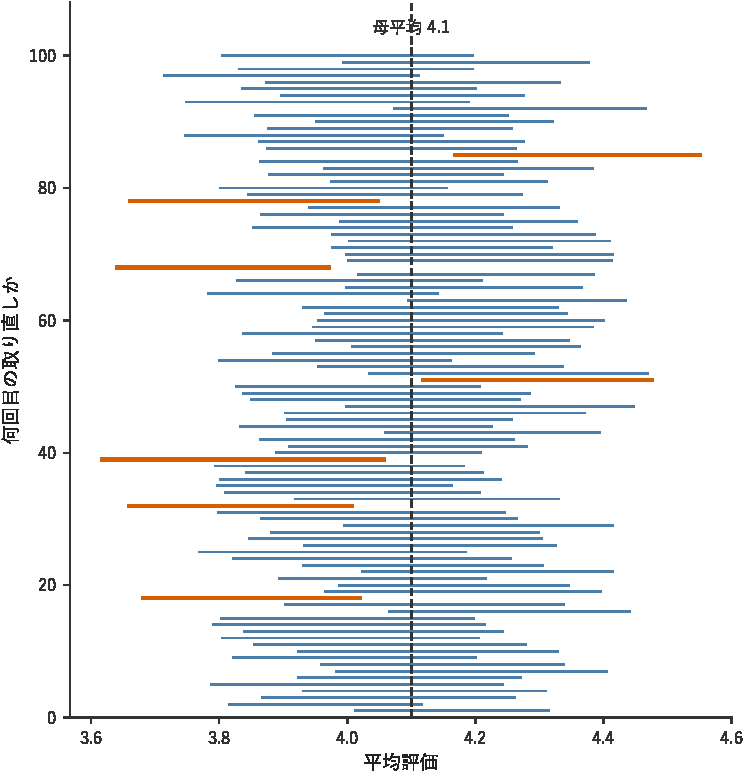
\includegraphics[width=0.8\linewidth]{../figures/output/ch05_ci_coverage.pdf}
      \caption{母平均4.1, 標準偏差0.7の母集団から50件の標本を取り, 95\%信頼区間を作る手順を100回繰り返した結果. 横棒の1本1本が1回分の区間を示す. 縦の破線は母平均4.1で, 動かない. 100本のうち93本(細い棒)は母平均を含み, 7本(太い棒)は外している.}
      \label{fig:ch04-ci-coverage}
    \end{figure}

    図を見ると, 100本の区間のうち93本は母平均の破線を含んでいるが, 7本は外してしまっている.
    きっかり95本にならないのは偶然で, この100回を別の機会にやり直せば, 含まれる本数は95本の前後に散らばる.

    図の棒は, どの1本も, 母平均を含んでいるか, 含んでいないかのどちらかで, 「95\%の確率で含んでいる」棒は1本もない.
    手元で作った $4.0$ から $4.4$ という区間も, 当たりか外れかのどちらかだ.
    ただ, 母平均を知らないかぎり, どちらなのかを確かめるすべはない.

    それなら, 手元の一本の区間など頼りにならないのではないか, と思えるかもしれない.
    それでもこの区間を信頼して使えるのは, 区間そのものが絶対だからではなく, 区間を作った手順のほうを信じているからだ.
    だから「95\%信頼区間」の95\%は, この区間に $\mu$ がある確率ではなく, 同じ手順で作った区間には, 100回に95回ほど母平均が入る, という意味だ.

  \subsection{区間があると何が変わるか}

    新しい薬の治験を行って, 「血圧を平均で 5\,mmHg 下げた」という結果が得られたとする.
    もしこの結果の95\%信頼区間が 2\,mmHg から 8\,mmHg だったとすれば, 取り直しのばらつきを考慮しても, おそらく少なくとも 2\,mmHg くらいは下がりそうだと見当がつく.
    医師もこれなら投薬の判断がしやすい.

    ところが, 同じ「平均 5\,mmHg 下がった」という結果であっても, 95\%信頼区間を計算してみたら $-1$\,mmHg から 11\,mmHg だったとしたらどうだろうか.
    区間の中にゼロやマイナスが含まれているということは, 本当の効果がまったくないことも, むしろ血圧が上がることも, 今回のデータからは否定できないということだ.
    そうなると, 軽々しく薬を使うわけにはいかなくなる.

    手元の標本平均が「5」であることだけを見ていたら, この二つの状況の違いには気づけない.
    幅があれば, 見積もりの値だけでなくその精度までわかるから, 過大な評価をうのみにしたり, 判断を誤ったりせずにすむ.

    区間の広さを決める手続きのうち, 何が数理的な必然で, 何が人間の選択なのかも整理しておこう.
    標本平均の分布が正規分布に近づくという事実は, 中心極限定理が保証するもので, 人間の都合で変えることはできない.
    一方で, 「100回に何回母平均が入るように作るか」という割合は, 計算する人間が目的に応じて選ぶものだ.
    この割合を\textbf{信頼水準}と呼ぶ.

    信頼水準を変えれば, 標準誤差に掛ける数字が変わる.
    \begin{itemize}
      \item 90\%なら $\pm 1.64 \times \mathrm{SE}$
      \item 95\%なら $\pm 1.96 \times \mathrm{SE}$
      \item 99\%なら $\pm 2.58 \times \mathrm{SE}$
    \end{itemize}

    99\%に設定すれば, 母平均を外してしまう区間は100回に1回ほどに減らせるが, そのかわり区間は左右に大きく広がってしまう.
    逆に90\%にすれば区間を狭く絞り込めるが, 10回に1回くらいは母平均を逃す区間ができるのを受け入れなければならない.
    世の中で95\%がよく使われるのは, 狭さと外しにくさの折り合いがほどよくつくという実用上の都合であって, 何か特別な理論的根拠があるわけではない.

    なお, 標本サイズが小さいときには, この「およそ2」という倍率をもう少し大きめに見積もる必要がある.
    本書では, 標本サイズがそこそこ大きくて倍率が2のままで足りる場合を考えていく.

  \subsection{映画の視聴回数を見積もる}

    映画80本のデータに戻ってみよう.
    手元の平均 $209.4$ 万回と標準誤差 $26.9$ 万回を使って, 95\%信頼区間を計算してみる.
    中心の $209.4$ から左右に $2 \times 26.9 = 53.8$ 万回だけ広げればよい.

    \[
      209.4 \pm 2 \times 26.9 \;\Rightarrow\; 155.6\;\text{万回} \;\sim\; 263.2\;\text{万回}
    \]

    およそ 156 万回から 263 万回という区間が得られた.
    手元の80本だけを計算した平均は確かに 209 万回だったが, 作品全体の本当の平均がそこからどれくらい外れうるかは, この区間を見ることで初めて見当がつく.

  \subsection{件数が増えると何が起きるか}

    前々章で, 星5つのレビューがついている商品があっても, レビューを書いたのがたったの1人だけなら素直に信じる気にはなれない, という話をした.
    その不安の正体も, 区間の広さとして捉え直すことができる.

    同じ平均 $3.8$, 標準偏差 $u = 0.9$ を示す商品であっても, レビューの件数 $n$ が異なると区間がどうなるかを見てみよう.
    \begin{itemize}
      \item $n = 5$ のとき: $\mathrm{SE} = 0.9 / \sqrt{5} \approx 0.40$ より, 区間は $3.8 \pm 0.80$ (3.0 〜 4.6)
      \item $n = 20$ のとき: $\mathrm{SE} = 0.9 / \sqrt{20} \approx 0.20$ より, 区間は $3.8 \pm 0.40$ (3.4 〜 4.2)
      \item $n = 100$ のとき: $\mathrm{SE} = 0.9 / \sqrt{100} = 0.09$ より, 区間は $3.8 \pm 0.18$ (3.62 〜 3.98)
    \end{itemize}

    手元の平均はどれも同じ $3.8$ だ.
    しかし, $n = 5$ のときの区間は $3.0$ から $4.6$ まで広がっていて, 凡作なのか名作なのか見分けがつかない.
    一方で $n = 100$ になれば, 区間は $3.6$ から $4.0$ 弱の狭い範囲に絞り込まれる.

    標準誤差の分母には $\sqrt{n}$ が入っている.
    そのため, 標本サイズを4倍に増やせば標準誤差は半分になり, 区間の広さも半分に縮む.
    たった数件の平均をそのまま信じるのがためらわれたのは, 計算された平均値そのものに欠陥があったからではなく, 背後にある区間があまりに広すぎて, 何も絞り込めていなかったからだ.

    新聞やテレビの世論調査で, 「内閣支持率45\%（$\pm 3$ポイント）」といった数字を見かけることがある.
    この「$\pm 3$ポイント」は, ここで計算した $\pm 2 \times \text{標準誤差}$ と同じものだ.
    同じ手順で作った区間には100回に95回ほど本当の値が入る. その作り方の信用を手がかりにして, 手元の一部のデータから全体の見当をつけている.

  \begin{mybox}{ここまででわかったこと}
    四段階の三つ目「ばらつきを見積もる」.

    \textbf{この章で言えるようになったこと}: 映画全体の平均視聴回数は, およそ $156$ 万回から $263$ 万回と見積もれた.
    偏りなく標本を取り, 同じ手順で区間を作れば, 100回に95回ほど本当の平均が入る.

    \textbf{まだ言えないこと}: 薬を飲んだ集まりと飲んでいない集まりのように, 二つの集まりを比べるときはどうだろうか.
    平均の差が, 取り直しのばらつきだけでも起きそうかどうかは, 差について確かめる必要がある.

    \textbf{前の章の見方がどう変わったか}: 標準誤差の $26.9$ 万回は, 取り直した平均がどれくらい動くかを表す数だった.
    そのぶん余裕を持たせると, 本当の平均がいそうな範囲を, 手順の信用とともに言えるようになった.
  \end{mybox}
